\chapter{Dane uczące}
\label{cha:dane}

Dane wykorzystane do uczenia i testowania stworzonego modelu zostały zaczerpnięte ze zbioru Treebank Wydźwięku (\textit{ang.  Polish Sentiment Treebank})\cite{treebank} w wersji 2.0. Zbiór uczący zawiera 2200 zdań o różnym stopniu złożoności, natomiast zbiór testowy składa się z 350 zdań. 

\section{Rozkład zdań}
\label{sec:rozklad}

Do plików z danymi tekstowymi dołączone są pliki \textit{parents} przedstawiające rozbiór gramatyczny zdań za pomocą drzew składniowych. Każde słowo ma przypisanego rodzica, czyli węzeł nadrzędny, natomiast korzeń drzewa posiada etykietę 0. W tabeli 3.1 przedstawiono przykładowe zdanie ze zbioru uczącego. Jak widać, w tym przypadku korzeniem drzewa jest słowo \textit{działali}.

\begin{table}[H]
\centering
\resizebox{\textwidth}{!}{%
\begin{tabular}{|l|c|c|c|c|c|c|c|c|c|c|}
\hline
\textbf{Pozycja w zdaniu} & 1                   & 2                & 3                   & 4           & 5             & 6                 & 7           & 8               & 9             & 10         \\ \hline
\textbf{Słowo lub znak}   & \textit{Zatrzymani} & \textit{wczoraj} & \textit{przestępcy} & \textit{od} & \textit{roku} & \textit{działali} & \textit{na} & \textit{własną} & \textit{rękę} & \textit{.} \\ \hline
\textbf{Rodzic}           & 3                   & 1                & 6                   & 6           & 4             & 0                 & 6           & 9               & 7             & 6          \\ \hline
\end{tabular}%
}
\caption{Przykładowe zdanie z wykorzystanego zbioru danych wraz z przypisanymi rodzicami.}
\label{table:bf-sa}
\end{table}

Dzięki takiemu rozbiorowi semantycznemu możliwe jest przedstawienie kontekstu słów w zdaniu w sposób zrozumiały dla sieci neuronowej.


\section{Etykiety}
Zdania w zbiorze danych są opatrzone etykietami wydźwięku (pliki \textit{labels}), gdzie \textit{-1} to opinia negatywna, \textit{0} \textendash \ neutralna, a \textit{1} pozytywna. Reprezentacja etykiet w zbiorze uczącym jest następująca: 54\% to etykiety pozytywne, natomiast 46\% \textendash \ negatywne. Ogólny wydźwięk zdania jest określany na podstawie etykiety korzenia drzewa, a także jego poddrzew. Jak widać na rys. 3.2, zdanie \textit{Widzę niepochlebne opinie o obsłudze, z którymi absolutnie się nie zgadzam.} zawiera człon \textit{widzę niepochlebne opinie o obsłudze}, który ma wydźwięk negatywny, dlatego został opatrzony etykietą \textit{-1}. Jednak negacja dalszej części zdania zmienia jego wydźwięk na pozytywny, dlatego korzeń drzewa ma ostetcznie etykietę \textit{1}. 
\label{sec:etykiety}
\begin{figure}[H]
    \centering
    \resizebox{\textwidth}{!}{%
    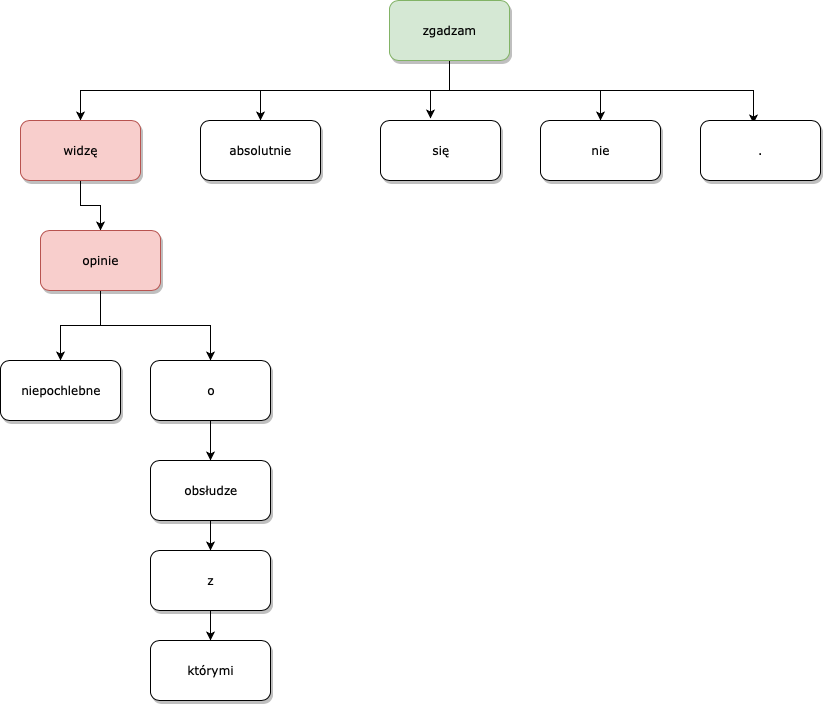
\includegraphics[clip]{labeled-tree.png}
    }%
    \caption{Drzewo zdania wraz z etykietami wydźwięku dla każdego poddrzewa.}
\end{figure}


